\section{Installation}
\label{sec:install}

In this chapter we explain how {\twodx} is installed on different operating systems. In order to ensure our easy-to-use policy we provide precompiled packages for Mac and some Linux distributions. After first listing all external dependencies we explain in details how to install the precompiled package on a Mac in \autoref{sec:install_pkg}. Subsequently we discuss the binary packages for Debian-like distributions (\autoref{sec:install_deb}) and for RedHeat-like Linux distribution (\autoref{sec:install_rpm}). Finally we provide a step-by-step manual on how to compile {\twodx} on your own machine.

\textbf{Important Note:} All the precompiled packages only run on $64$ bit machines. If you are still using a $32$ bit operating system you have to compile {\twodx} yourself as described in \autoref{sec:install_source}.

\textbf{Login required!} Downloading {\twodx} requires that you are logged in on our homepage. Creating an account can be done at anytime and for free. We use the login mechanism for tracking all users and to inform you about new {\twodx} versions and upcoming events. We will not spam your mail account and will treat your informations with all the required privacy.

\subsection{External Dependencies}
\label{sec:2dxdeps}
\index{Dependencies}
{\twodx} depends on some third-party programs which have to be installed on your system. 

\begin{itemize}
	\item \textbf{TCSH:} Some of our scripts require an alternative C-shell called tc-shell. We advise to install this shell by means of your native package manager, e.g. \texttt{port}, \texttt{apt-get} or \texttt{yum}. For further information we refer to \url{http://www.tcsh.org/Welcome}.
	\item \textbf{CCP4:} {\twodx} uses \texttt{CPP4} in order to generate merged maps of the protein. The software can be downloaded from \url{http://www.ccp4.ac.uk/download.php}. Please follow their installation guide. Please install CPP4 into \texttt{/usr/local/ccp4}.
	\item \textbf{Chimera:} 3D density maps can be visualized in a powerful way by means if Chimera. You find all the required information and packages on \url{http://www.cgl.ucsf.edu/chimera/}.
	\item \textbf{Spider:} If you would like to have density maps larger than $2\times 2$ unit cells {\twodx} generates them for you with Spider. We refer to \url{http://www.wadsworth.org/spider_doc/spider/docs/spider.html}. To ensure that {\twodx} finds Spider you should install the software into \texttt{/usr/local/spider}. In fact {\twodx} searches for an executable file called \texttt{spider.exe} in the folder mentioned before.
\end{itemize}

\newpage

\subsubsection{\texttt{CCP4} on Linux}
As we had serious issues in context of installing and using \texttt{ccp4} on Linux, we provide a walkthrough which worked on our systems. 
\begin{enumerate}
	\item Download the latest version (tested with \texttt{ccp4-6.3.0})
	\item Extract the downloaded archive
	\item Move the generated folder to \texttt{/usr/local/ccp4-6.3.0}
	\item Go to \texttt{/usr/local/ccp4-6.3.0} and run the \textit{BINARY.setup} script as root
	\item Generate a symbolic link to \texttt{/usr/local/ccp4} by typing: \newline \texttt{sudo ln -s /usr/local/ccp4-6.3.0 /usr/local/ccp4}
\end{enumerate}

\newpage


\subsection{Downloading {\twodx}}
\index{Download}
{\twodx} is freely available under the General GNU public license (GPL). Please use the following page for downloading {\twodx} \url{http://www.2dx.unibas.ch/download/2dx-software}. In general we offer two different versions to download. On one hand you can download the latest version of {\twodx} which is a snapshot of the source code repository at midnight (i.e. \textit{nightly build}). Although we give our best we can not guaranty that this version, which contains all the latest features, does alway works perfectly. On the other hand we offer previous versions of {\twodx}, which should be more stable but do not contain the latest fixes and features. 

\textit{Which version should you download?} In general we advise to use the nightly build version from \url{http://www.2dx.unibas.ch/download/2dx-software/2dx-nightly-build}. This folder contains for different archives:
\index{Nightly build}

\begin{itemize}
	\item \textbf{2dx\_nightly\_build\_OSX.pkg} is an easy to install package for Mac. We tested this installer on OSX10.6 (Leopard), OSX10.7 (Lion) and OSX10.8 (Mountain Lion). Using this package is the easiest way to install {\twodx} on a Mac in general. You find a detailed manual in \autoref{sec:install_pkg}.
	\item \textbf{2dx\_nightly\_build\_Linux.deb} is a precompiled binary package for debian-like distributions like Ubuntu, Mint or Debian. Further information can be found in \autoref{sec:install_deb}.
	\item \textbf{2dx\_nightly\_build\_Linux.rmp} is a binary archive for RedHeat, Fedora or Scientific Linux. A walkthrough the installation is given in \autoref{sec:install_rpm}.
	\item \textbf{2dx\_nightly\_source.tar.gz} should be used in case you want or have to compile {\twodx} on your machine yourself. Note that this compilation, which is described in \autoref{sec:install_source}, does not depend on the used operating system.
\end{itemize}

You also find all the older versions of {\twodx} in our download domain. If you feel more comfortable with installing a older but potentially more stable version you also can download the outdated archives. The installation itself is the same as for the nightly build.

\subsection{Installation on Mac}
\index{Installation!On Mac}
\label{sec:install_pkg}
The installation on a Mac is straightforward as you just have to run the installer. In order to install you need administrator privileges on your machine. If you don't have them please contact your system administrator. The following steps are required to install the package on your Mac.

\begin{enumerate}
	\item (Only required on OSX10.8 Mountain Lion) Apple's new security policy per default allows you to install software just from the App Store. To be able to install {\twodx} you have to allow the installation from other sources as just the App Store. This can be done under "System Preferences > Security \& Privacy > General > Adcanced..." as shown in \autoref{fig:mlion_settings}.
	
	\begin{figure}[H]
		\centering
		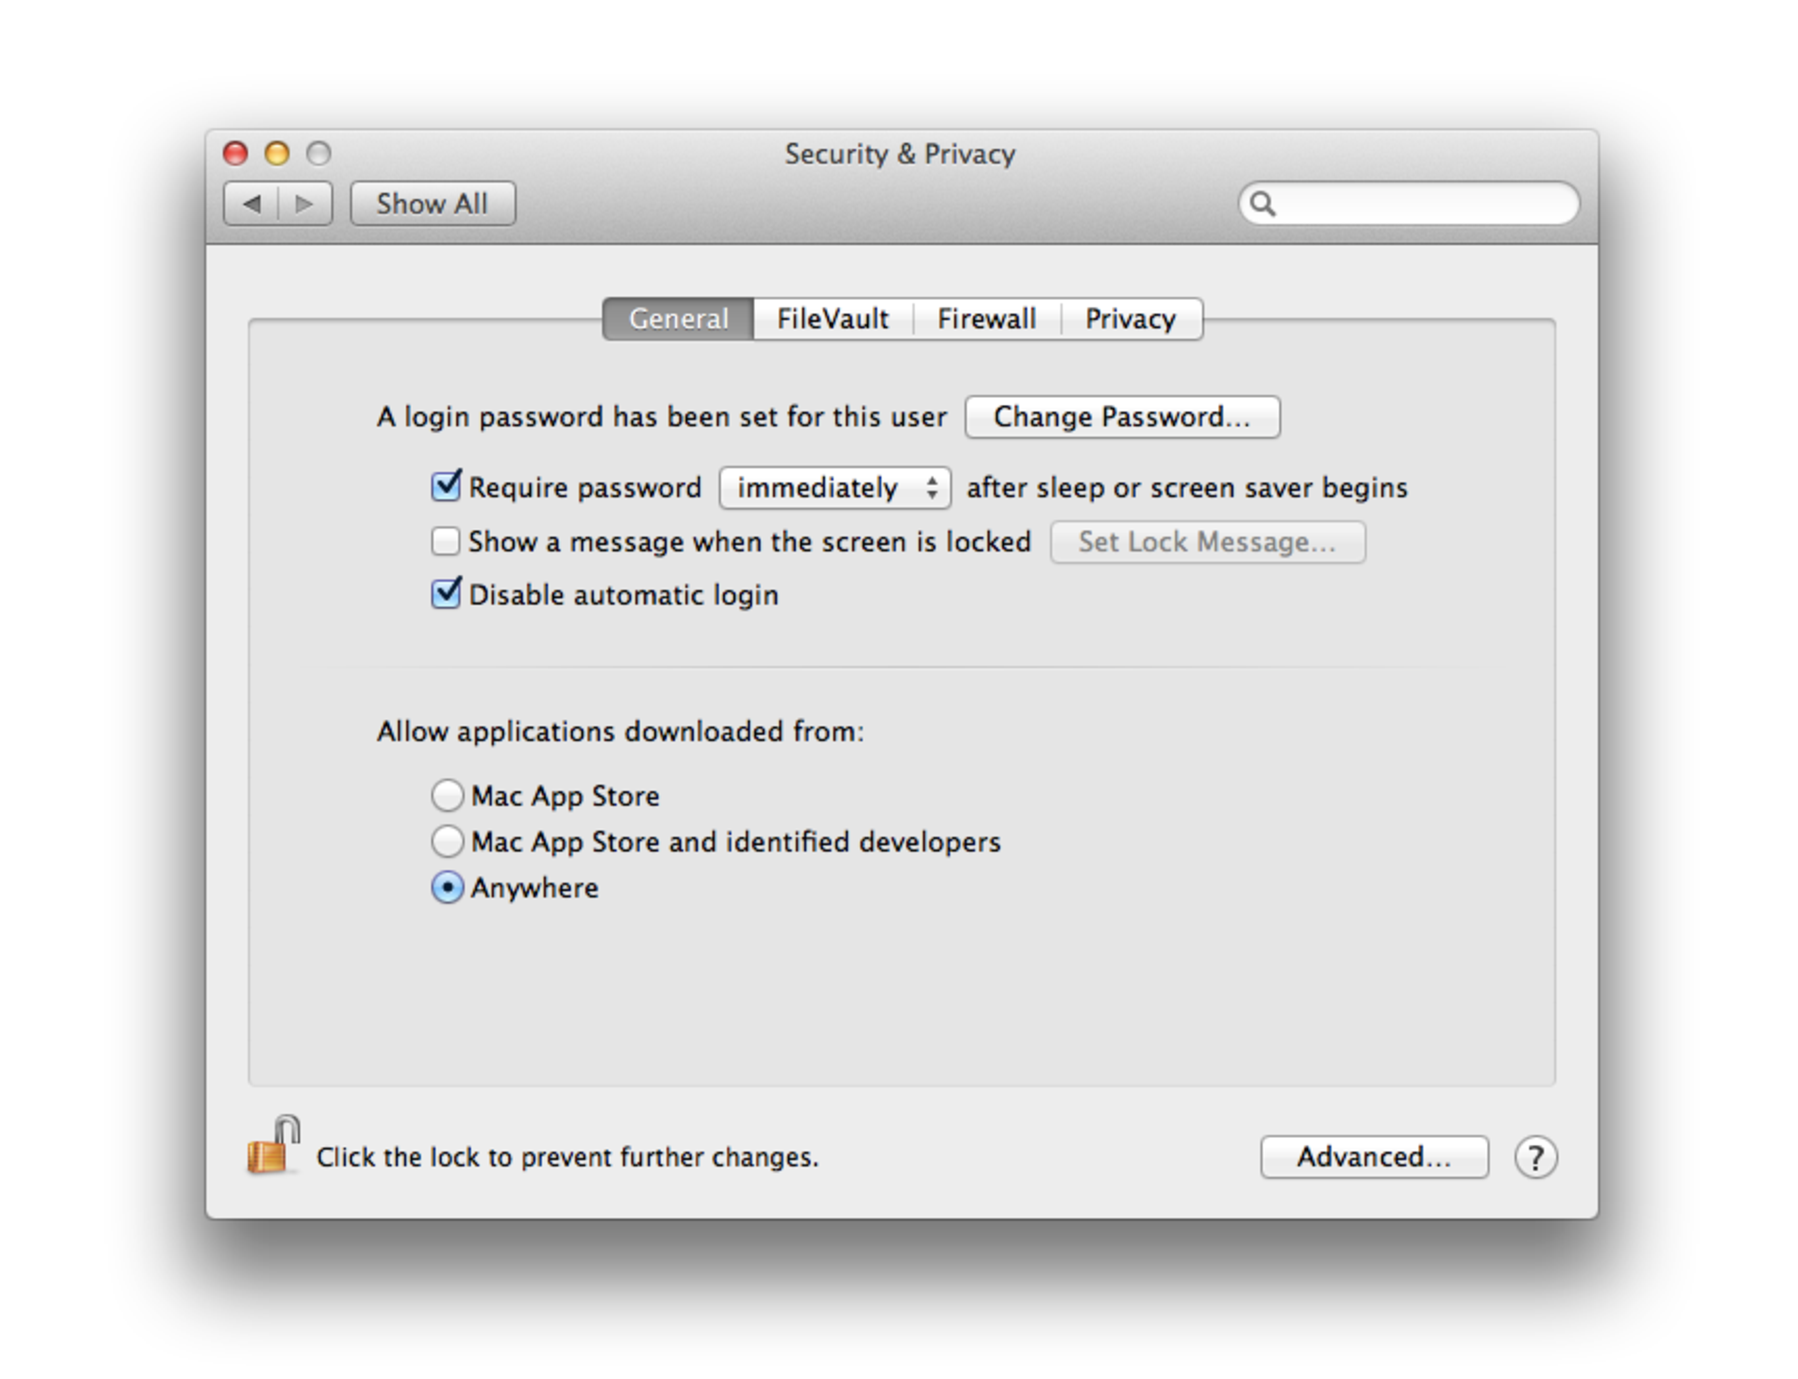
\includegraphics[width=.85\textwidth]{mlion_setting.pdf}
		\caption{Mountain Lion Security Settings}
		\label{fig:mlion_settings}
	\end{figure}
	
	\item After downloading double-click on the downloaded package. This will launch the installation dialog shown in \autoref{fig:installer_mac}.
	
	\begin{figure}[H]
		\centering
		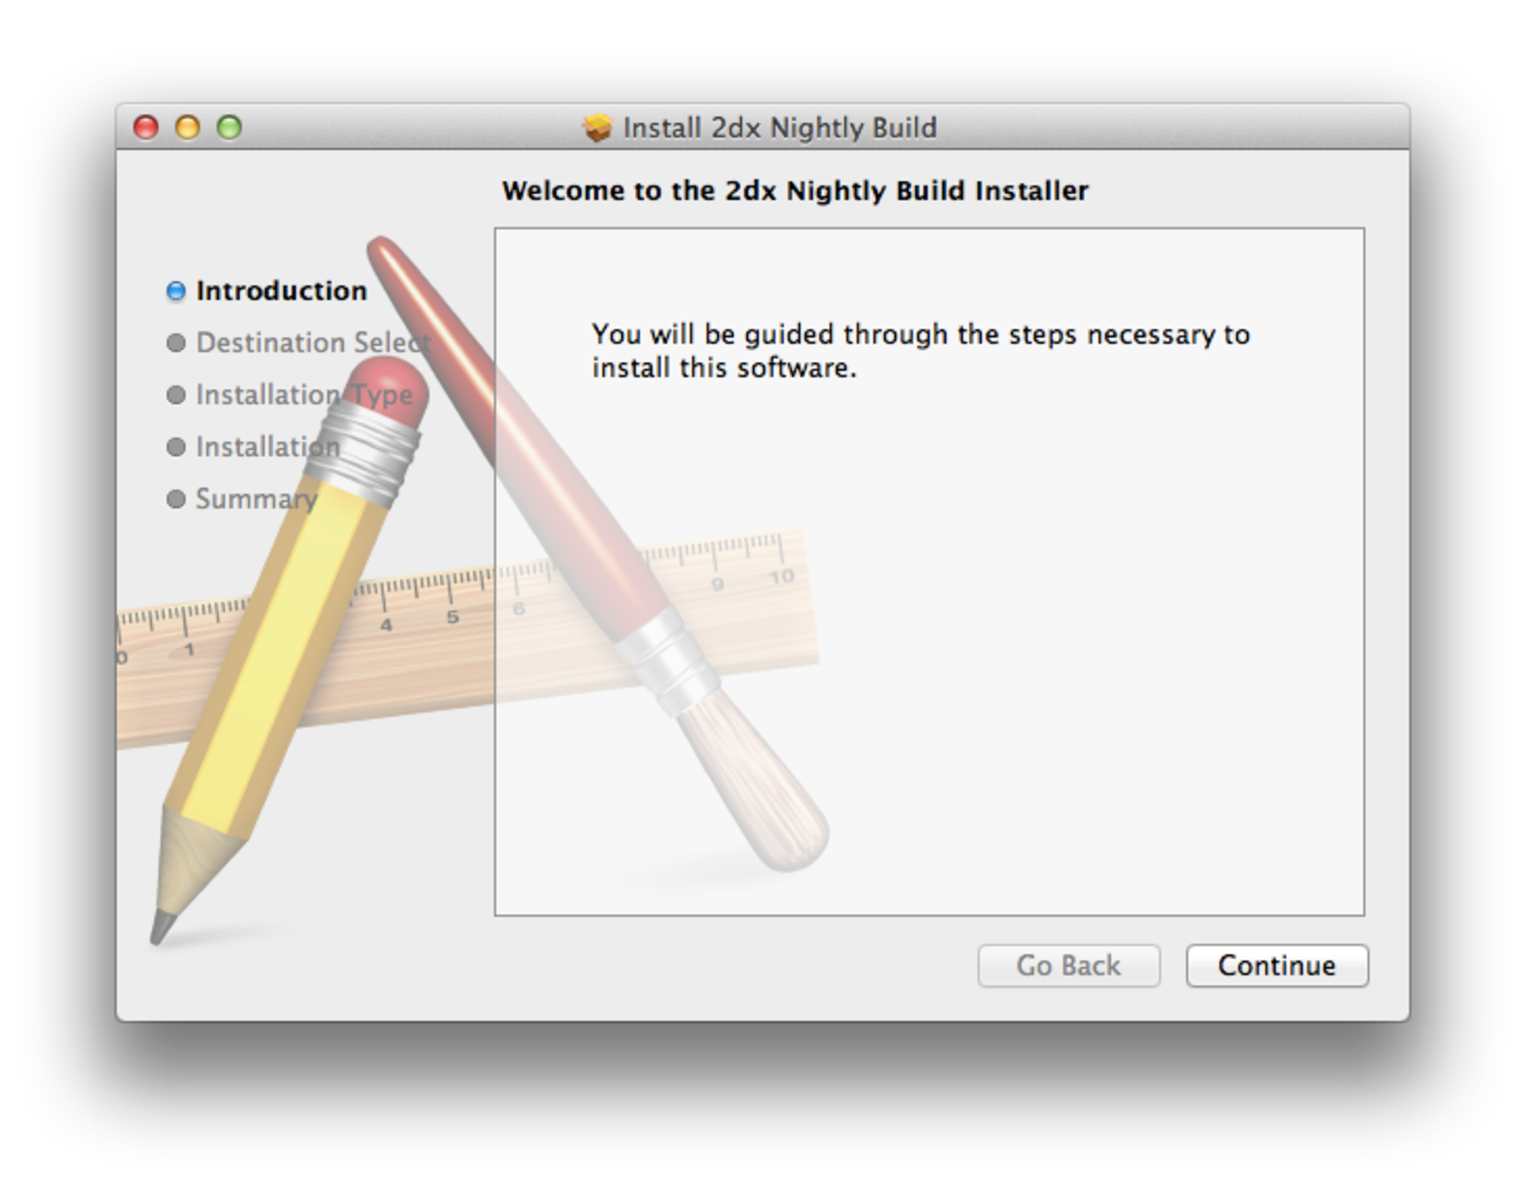
\includegraphics[width=.85\textwidth]{installer_mac.pdf}
		\caption{{\twodx} installer on Mac}
		\label{fig:installer_mac}
	\end{figure}
	
	\item The first window tells you that this installer will guide you trough the installation process. You reach the next page by clicking on "continue"..
	\item Now you are ask where you want to install the software. The simplest way is to click "continue" and the software will be installed in the default location (\texttt{/opt/2dx}) and can be run by all the users of the computer.
	\item The following screen shows you a summary of the planed installation. A click on the "install" button will launch the installation process. Usually you are ask to enter the administrator password (\autoref{fig:mac_admin}) before the software is installed.
	
	\begin{figure}[H]
		\centering
		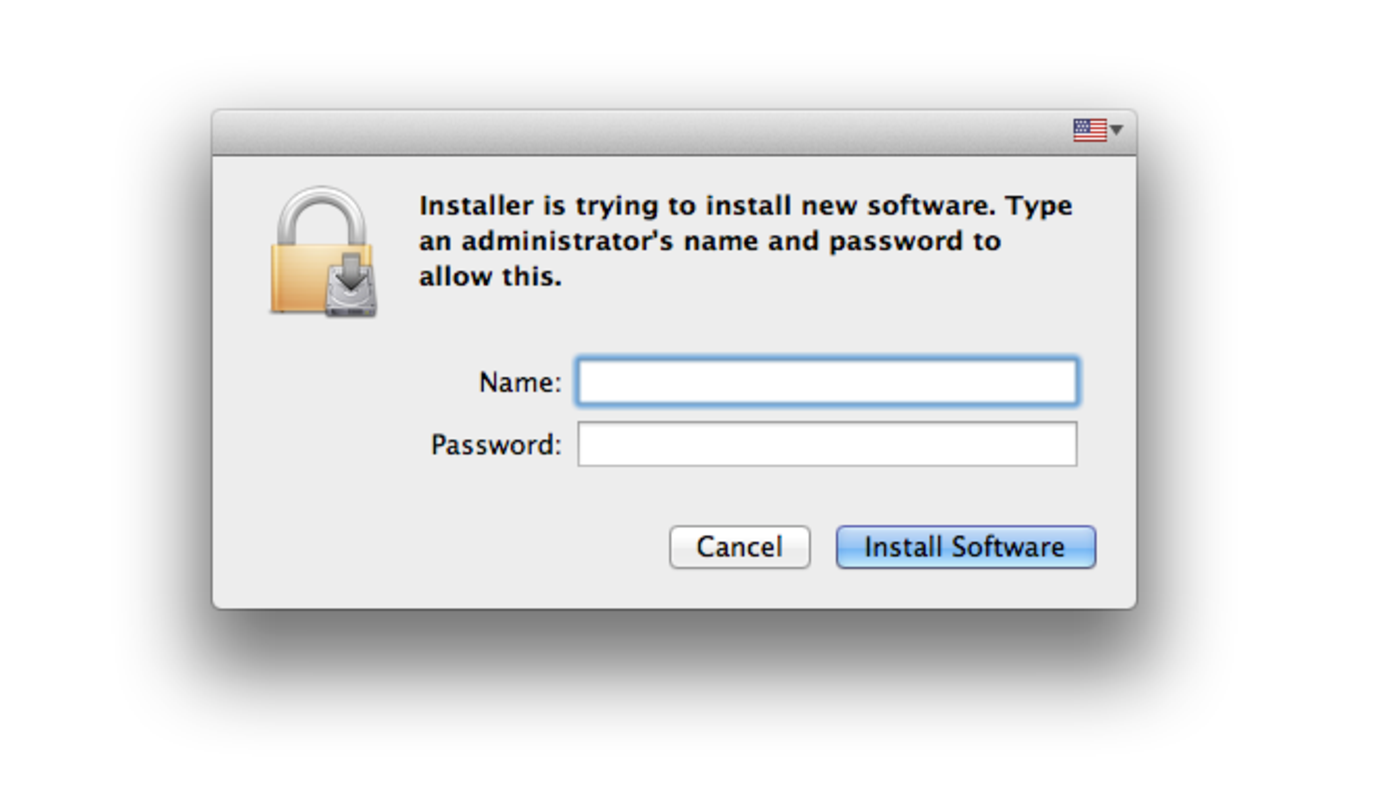
\includegraphics[width=.85\textwidth]{mac_admin.pdf}
		\caption{Installer asking for administrator privileges on a Mac}
		\label{fig:mac_admin}
	\end{figure}
	
	\item Once you entered the correct administrator password the installation is performed and you see a growing status bar.
	\item If everything worked well the installer tells you that the installation was successful (\autoref{fig:mac_installation_done}). In the mean time the Application folder is opened and you should find a {\twodx} icon.
	
	\begin{figure}[H]
		\centering
		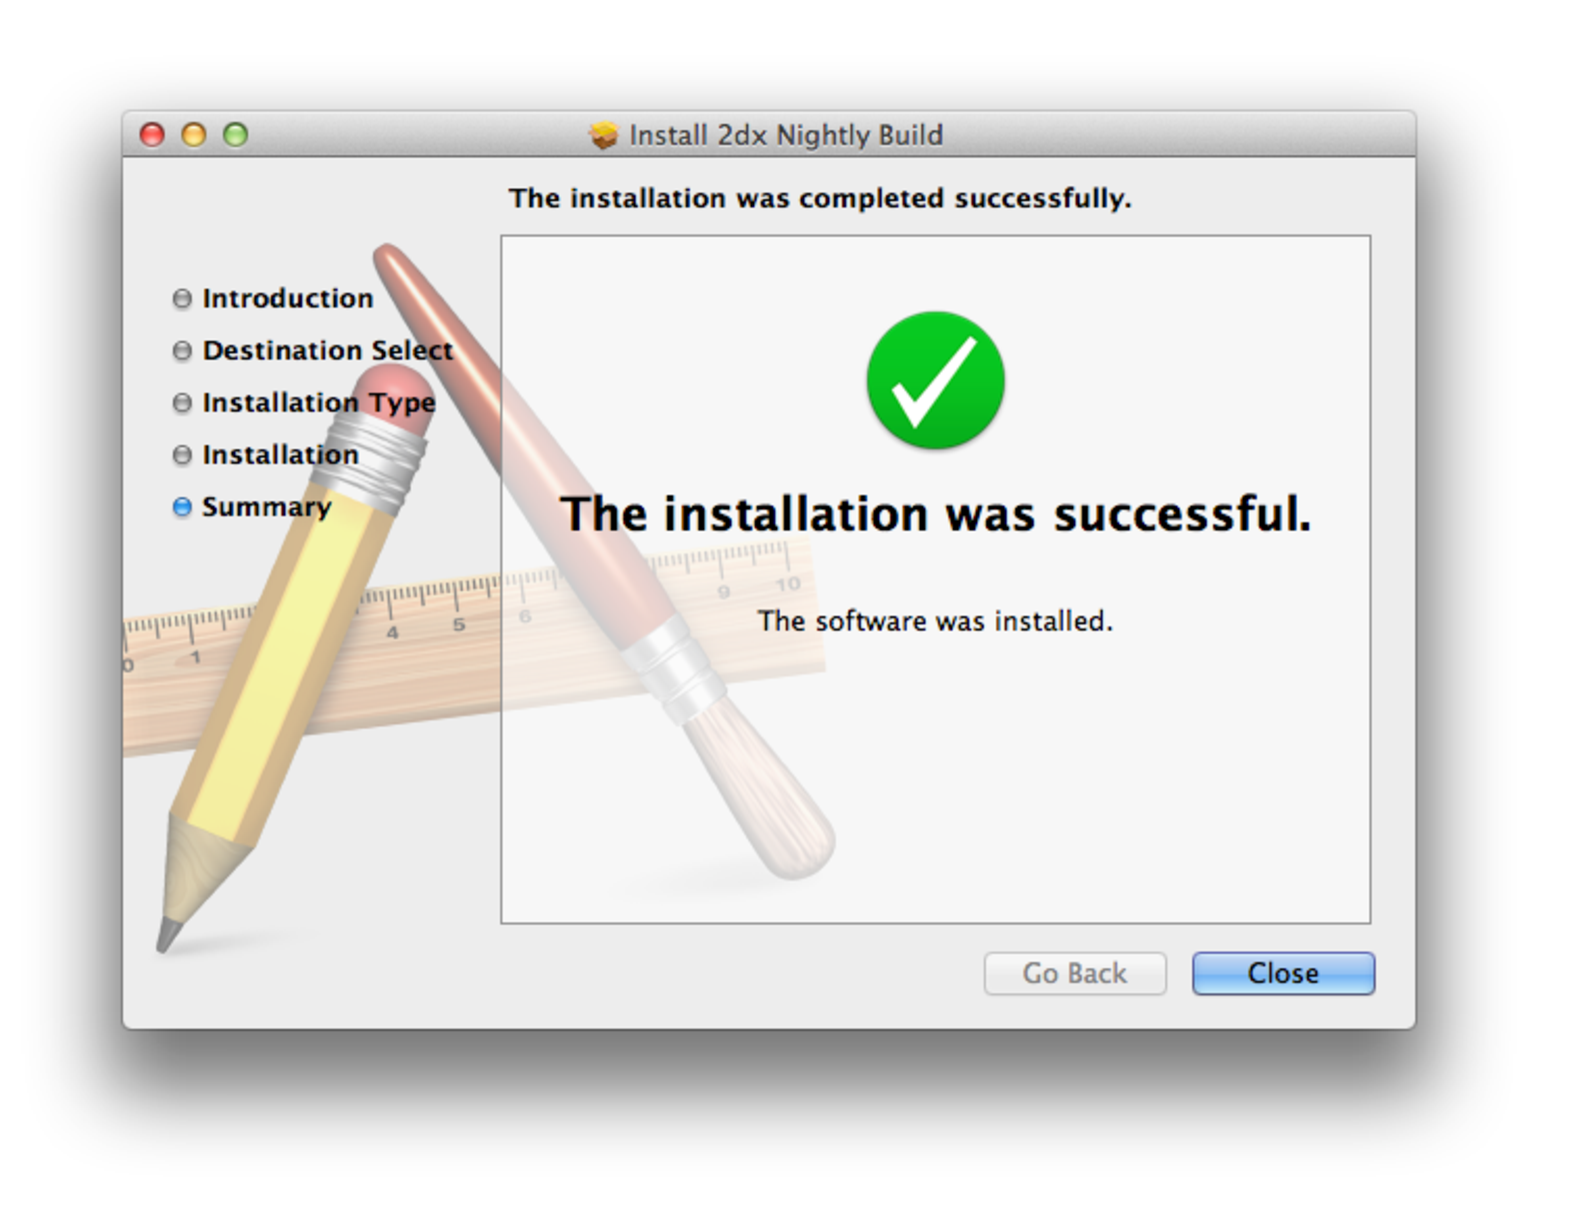
\includegraphics[width=.85\textwidth]{mac_installation_done.pdf}
		\caption{Successful installation on Mac}
		\label{fig:mac_installation_done}
	\end{figure}
	
	\item You can launch {\twodx} by double-clicking on this icon.
\end{enumerate}

\newpage

\subsection{Installation on Linux (Ubuntu)}
\index{Installation!On Ubuntu}
\label{sec:install_deb}
Due to some technical problems\footnote{upgrade of libc6 to version 2.14 which is not compatible with all earlier versions} we can just deliver a binary package which works on Ubuntu-12.04. In case you can not upgrade your distribution you can either compile {\twodx} yourself (\autoref{sec:install_source}) or upgrade libc6 to version 2.14.xx on your older Ubuntu. Note that the described update is not officially supported and we don't give any warranty.

\textbf{Note} that \texttt{tcsh} is not resolved automatically and that you are responsible for installing this additional shell yourself (\autoref{sec:2dxdeps})

Below you find a step-by-step walkthrough the installation on a $64$ bit Ubuntu-12.04. 

\begin{enumerate}
	\item If you download the package \textbf{2dx\_nighlty\_build\_Linux.deb} from our homepage Firefox asks you what you what you want to do with the downloaded file (\autoref{fig:ubuntu_download}). The easiest way is to open the package directly with the Ubuntu Software Center by means of clicking "ok" in the shown dialog. Alternatively you can also download the package and then double-click on it.

	\begin{figure}[H]
		\centering
		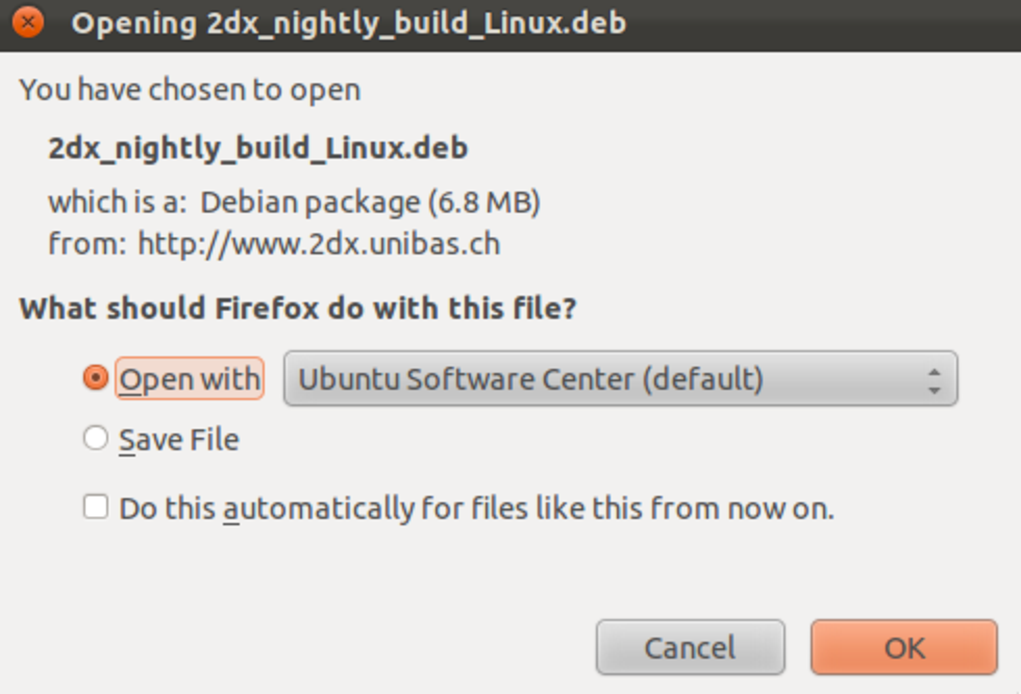
\includegraphics[width=.65\textwidth]{ubuntu_download.pdf}
		\caption{Download dialog on Ubuntu}
		\label{fig:ubuntu_download}
	\end{figure}
	
	\item After opening the package with the Ubuntu Software Center you get the window shown in \autoref{fig:ubuntu_installler} where you can see a summary of our package.
	
	\begin{figure}[H]
		\centering
		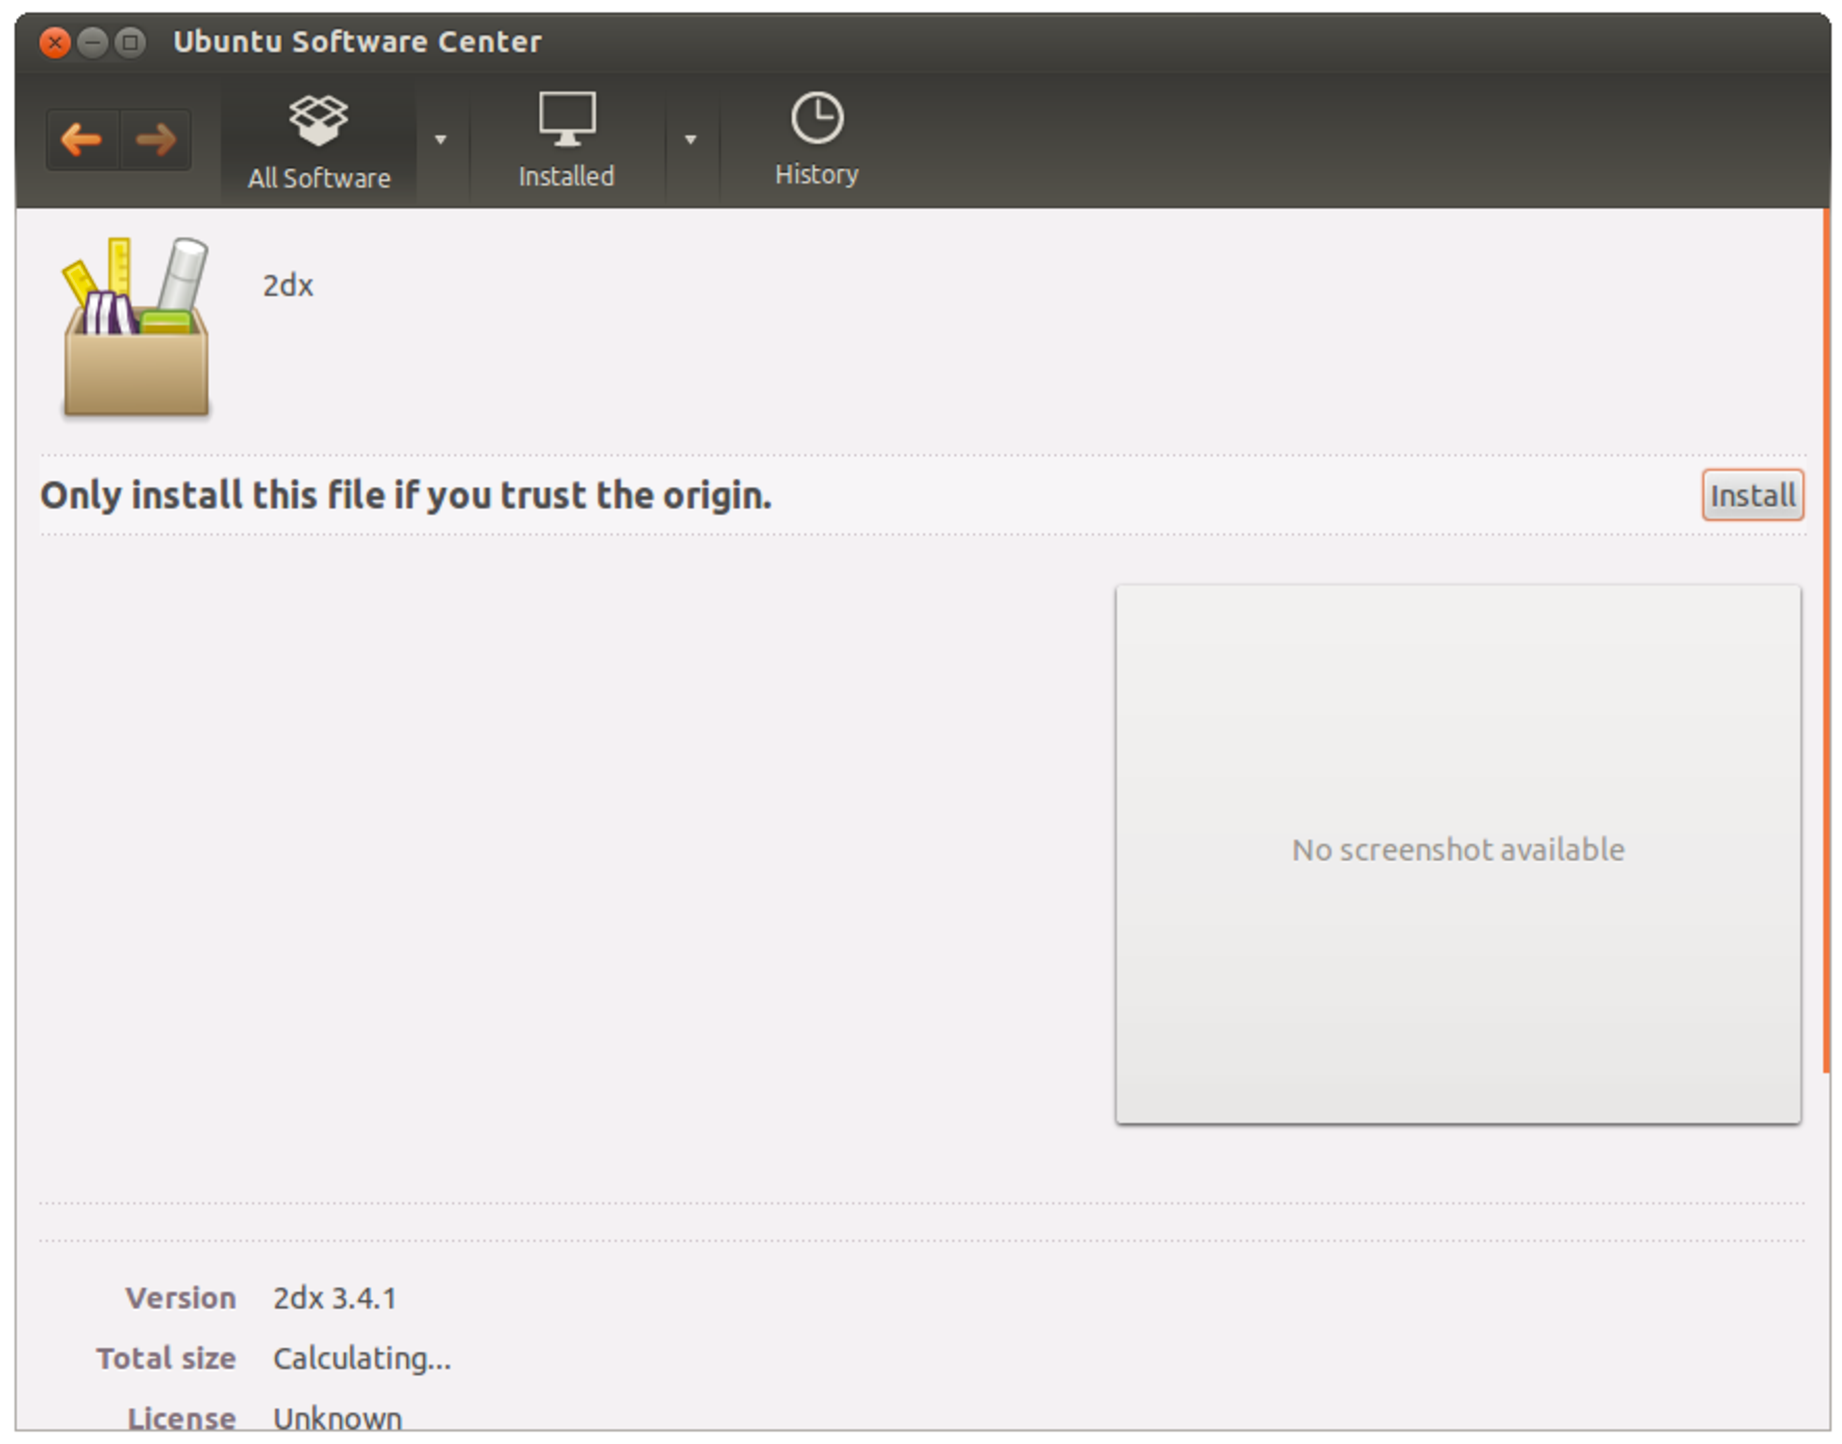
\includegraphics[width=.85\textwidth]{ubuntu_install.pdf}
		\caption{{\twodx} installation with Ubuntu's Software Center}
		\label{fig:ubuntu_installler}
	\end{figure}
	
	\item Clicking on "install" starts the installation process. For security reasons you are asked for the \texttt{sodu} password as normal users are not allowed to install software. Please enter the required password in the window shown in \autoref{fig:ubuntu_admin}.
	
	\begin{figure}[H]
		\centering
		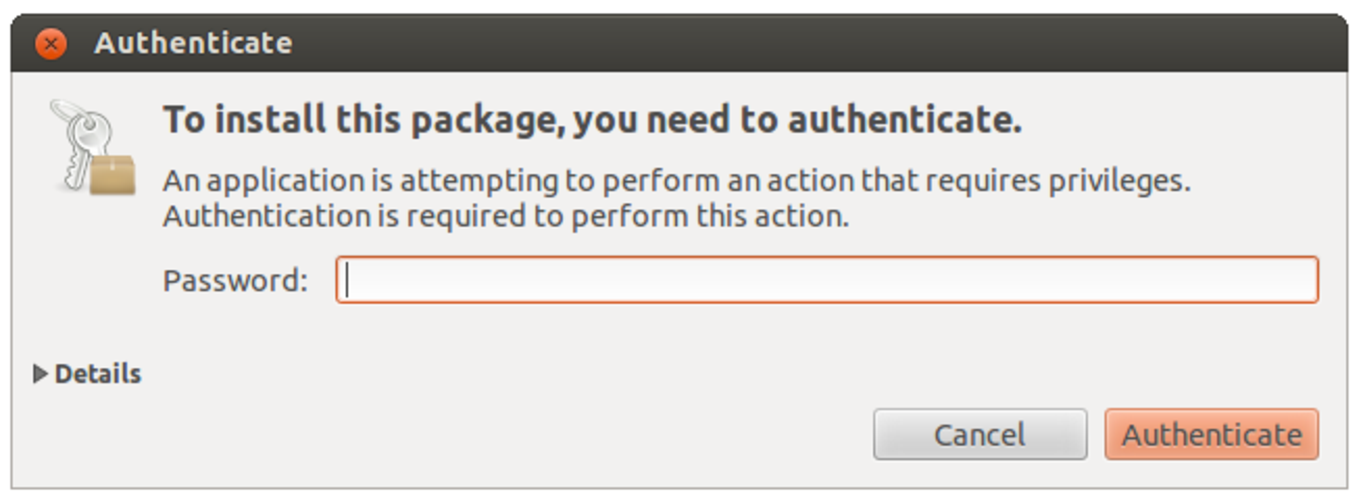
\includegraphics[width=.85\textwidth]{ubuntu_admin.pdf}
		\caption{Ubuntu's Software Center asking for administrator privileges}
		\label{fig:ubuntu_admin}
	\end{figure}
	
	\item After successfully installing {\twodx} you will find a {\twodx}-icon under the "Education" menu entry (\autoref{fig:ubuntu_launch}). You now can start {\twodx} by simply clicking on this icon. 
	
	\begin{figure}[H]
		\centering
		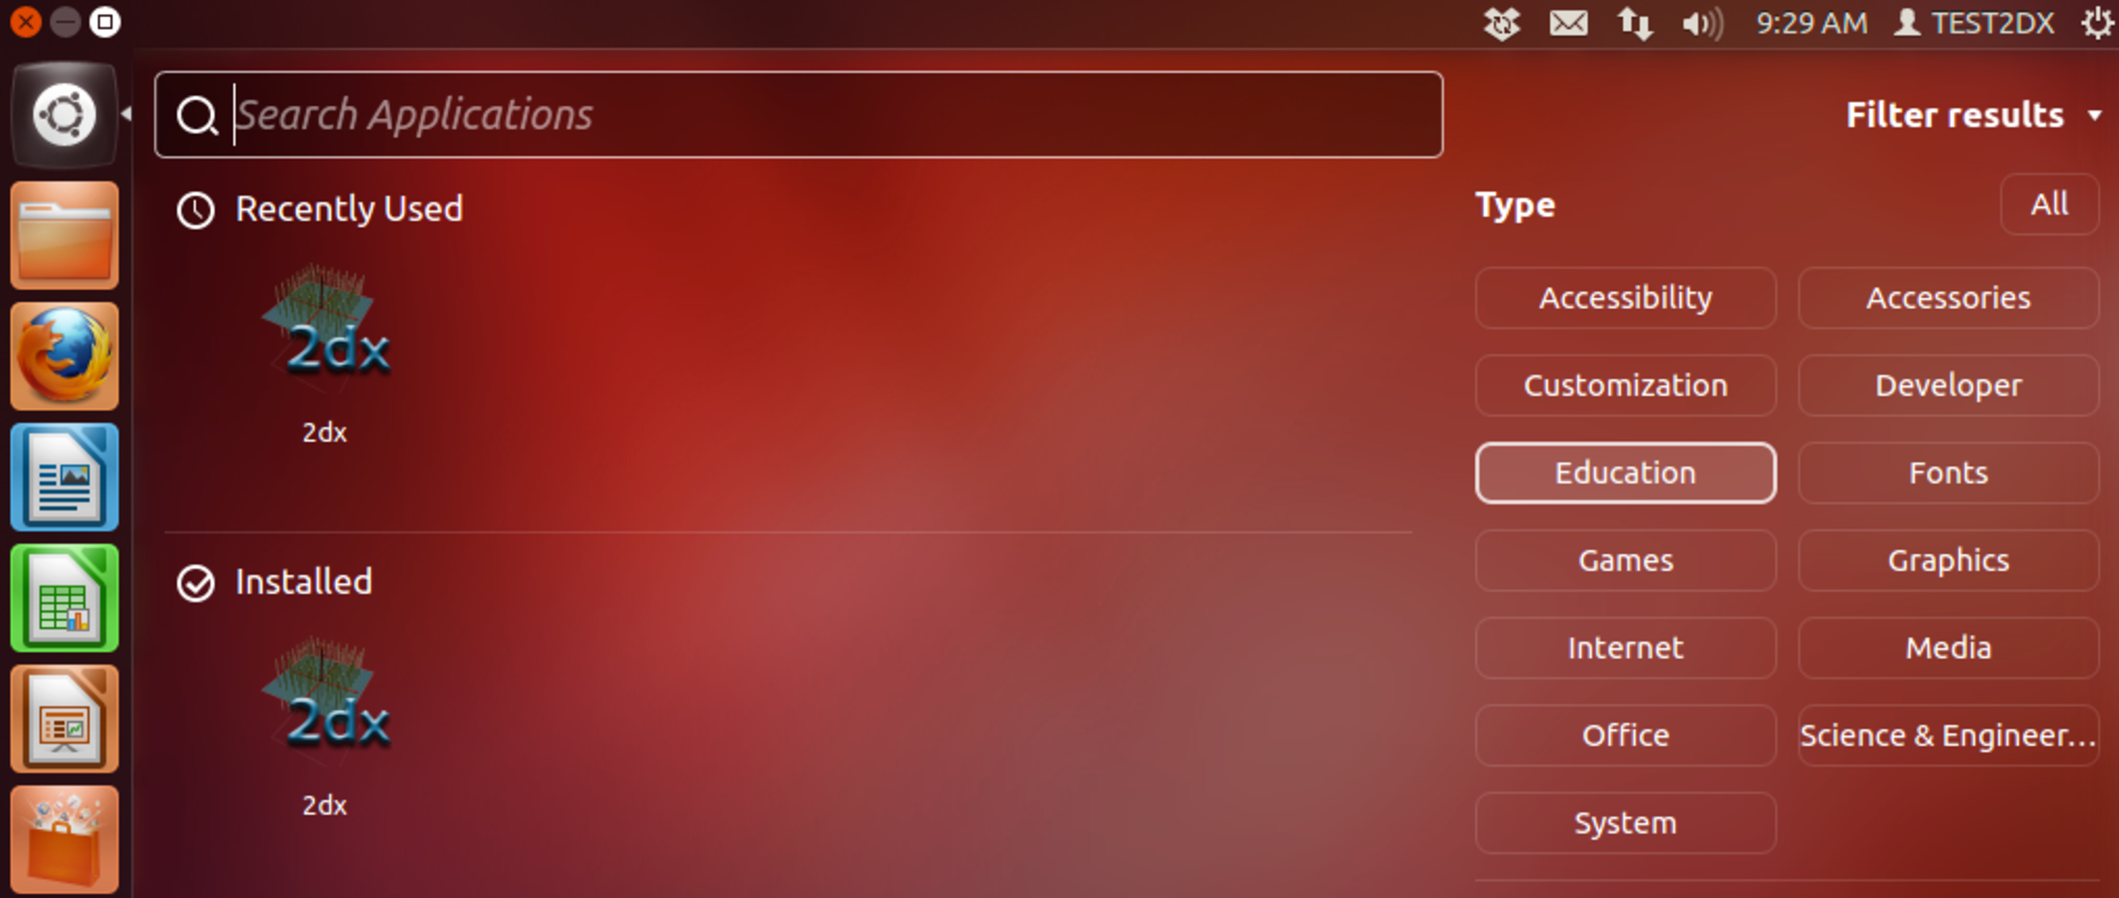
\includegraphics[width=.85\textwidth]{ubuntu_launch.pdf}
		\caption{Launching {\twodx} on Ubuntu}
		\label{fig:ubuntu_launch}
	\end{figure}
	
	Additionally we also install {\twodx}\texttt{\_image} which is used for single image processing. In general you should not open {\twodx}\texttt{\_image} directly yourself as {\twodx}\texttt{\_merge} will open it for you with the correct parameters.

\end{enumerate}

\subsection{Installation on Linux (Fedora)}
\index{Installation!On Fedora}
\label{sec:install_rpm}
The following manual guides you through the installation process on RedHeat-like distributions. We tested the installation on Fedora 16 and Fedora 17 but we don't see any reason why it should not work on other similar platforms. 

\begin{enumerate}
	\item If you download the package \textbf{2dx\_nighlty\_build\_Linux.rpm} from our homepage Firefox asks you what you want do do with the downloaded file (\autoref{fig:fedora_download}). The easiest way to launch the installation process of the package directly is clicking on the "ok" button. Alternatively you can also download the package and then double-click on it.
	
	\begin{figure}[H]
		\centering
		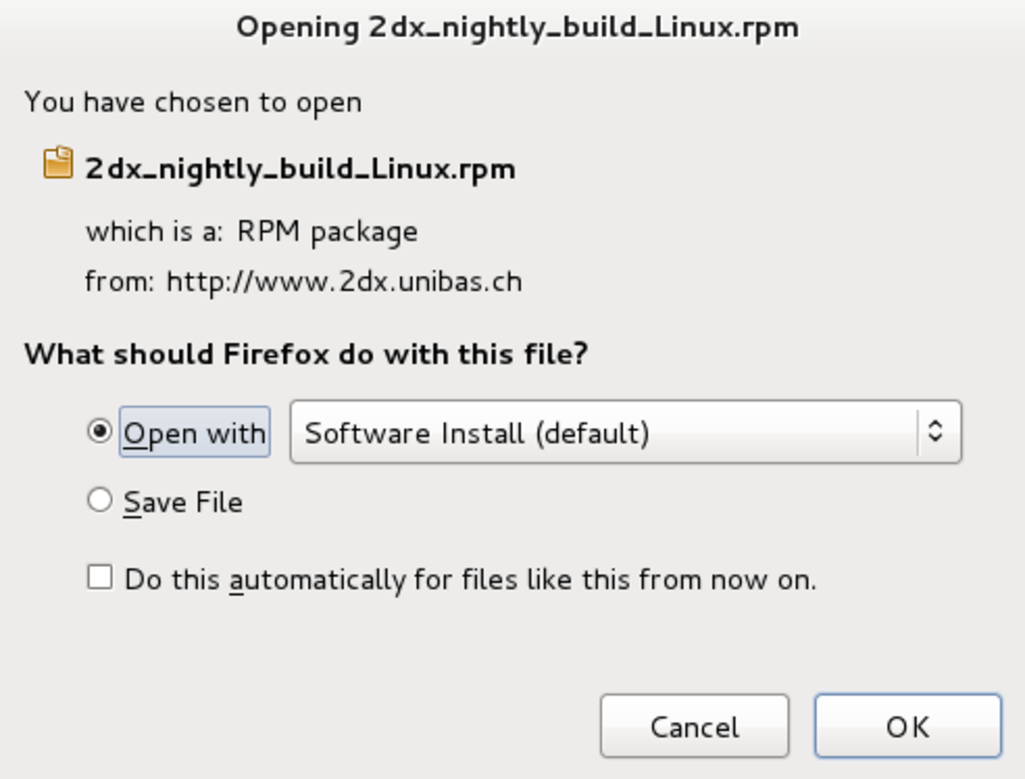
\includegraphics[width=.85\textwidth]{fedora_download.pdf}
		\caption{Download dialog on Fedora}
		\label{fig:fedora_download}
	\end{figure}
	
	\item Next you are asked whether you really want to install the packages (\autoref{fig:fedora_install}). 
	
	\begin{figure}[H]
		\centering
		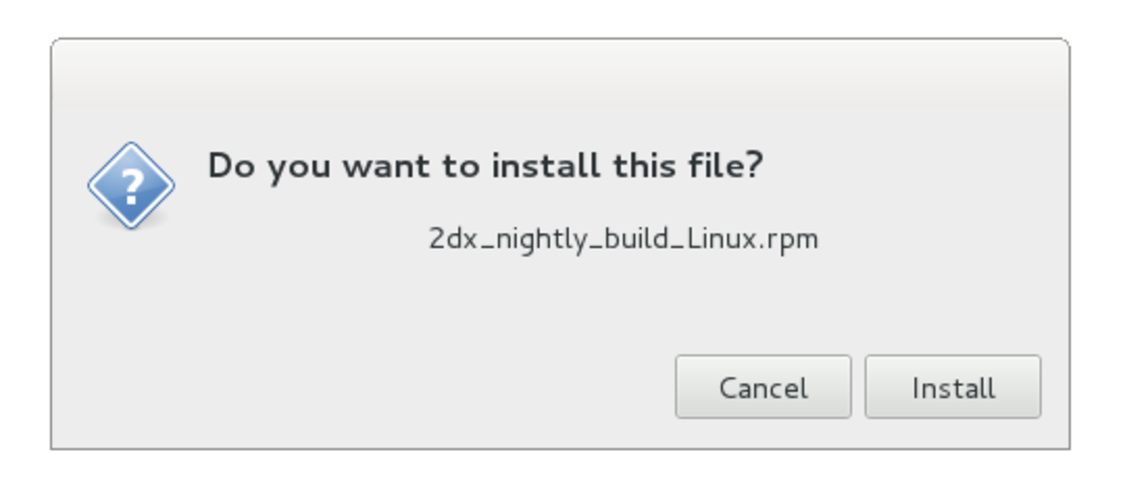
\includegraphics[width=.65\textwidth]{fedora_install.pdf}
		\caption{Installation dialog on Fedora}
		\label{fig:fedora_install}
	\end{figure}
	
	Clicking on "install" brings you to the next step.
	
	\item Before the installation process is launched you have to enter the \texttt{sudo} password as shown in \autoref{fig:fedora_admin}. Please note that if you use the native package manager all dependencies will be installed automatically. If you use another package installer you probably have to install some dependencies manually before the installation of {\twodx} will be launched.
	
	\begin{figure}[H]
		\centering
		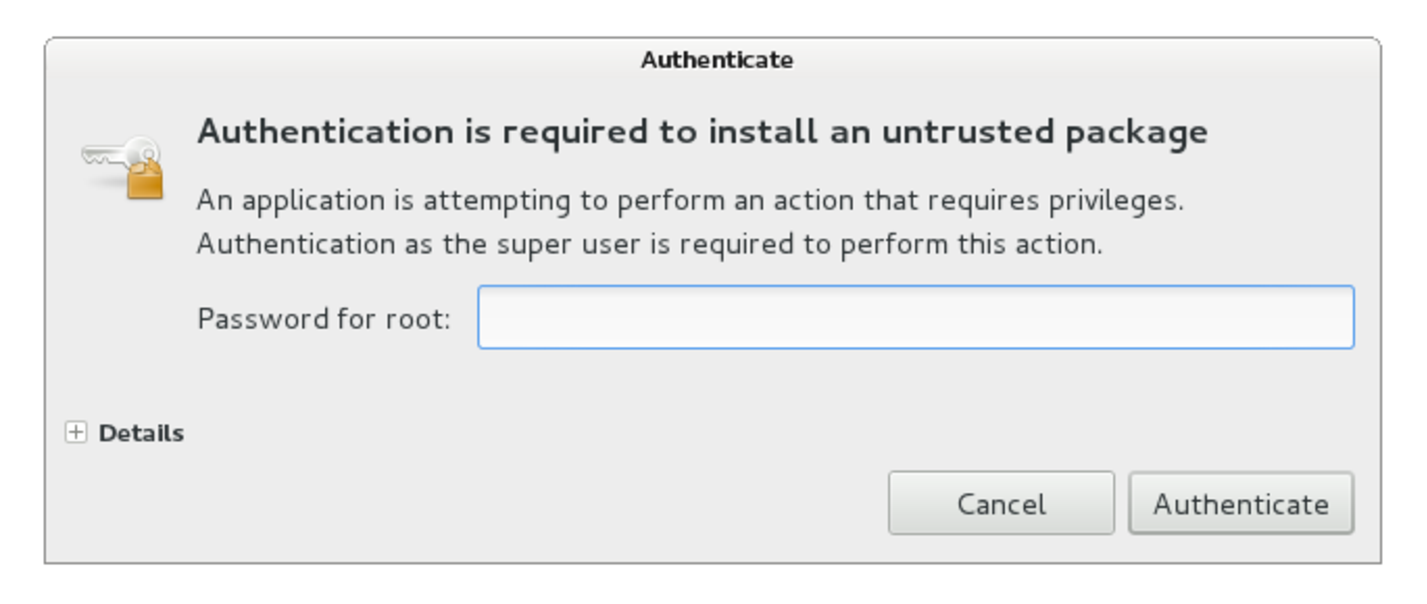
\includegraphics[width=.75\textwidth]{fedora_admin.pdf}
		\caption{Fedora installer asking for the root password}
		\label{fig:fedora_admin}
	\end{figure}
	
	\item After the successful installation you will find a {\twodx}-icon under the "education" menubar as shown in \autoref{fig:fedora_icon}.
	
	\begin{figure}[H]
		\centering
		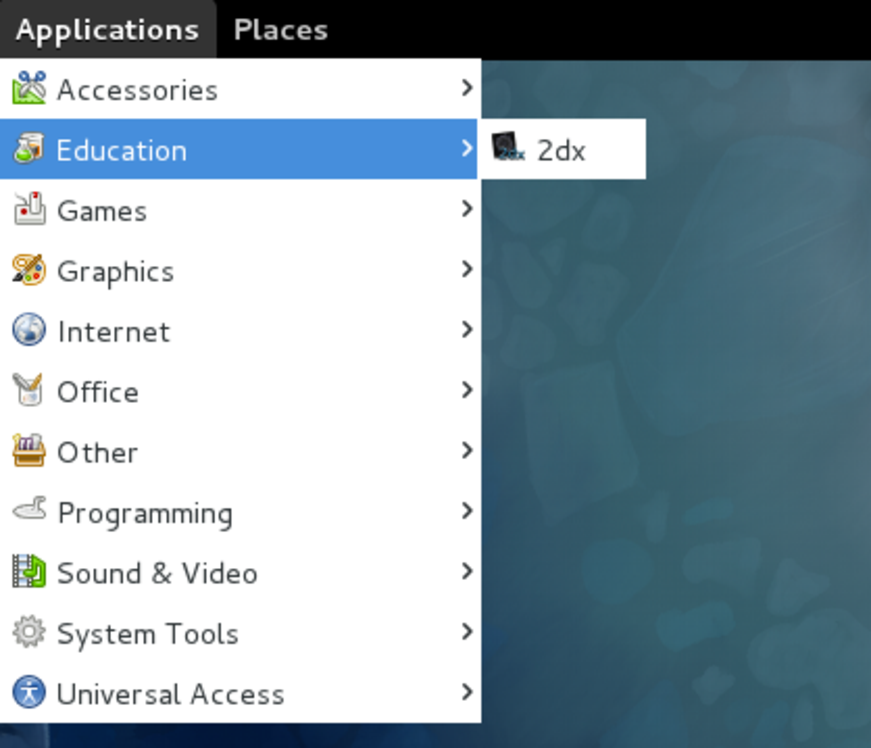
\includegraphics[width=.75\textwidth]{fedora_icon.pdf}
		\caption{Launching {\twodx} on Fedora}
		\label{fig:fedora_icon}
	\end{figure}
	
	Additionally we also install {\twodx}\texttt{\_image} which is used for single image processing. In general you should not open {\twodx}\texttt{\_image} directly yourself as {\twodx}\texttt{\_merge} will open it for you with the correct parameters.
	
\end{enumerate}

\newpage

\subsection{Compiling from source}
\index{Compilation from source}
\label{sec:install_source}
In this section we explain how to compile {\twodx} on your own machine, which always slightly depends on your specific operating system and the version of the installed software. Thus we only insure that our manual works for Ubuntu 12.04, Fedora 17 and OSX.10.7. Probably some dependencies slightly change for other platforms but the basic concept stays the same. An additional challenge is to know the correct linux specific package name. We state all dependencies on Linux in term of the Ubuntu/Debian naming convention and we give some additional hints for RedHeat-based systems.

For OSX we suggest that you install the dependencies via macports (\url{http://www.macports.org}). 

The only supported compilers are \texttt{gcc} and \texttt{icc}. On mac please install \texttt{gcc4X} via macports and activate the installed compiler with \texttt{sudo port select --set gcc mp-gcc4X}. Note that \texttt{X} stands for the particular version you installed. The compilation process was successfully tested with \texttt{gcc48} and \texttt{gcc49}.

\subsubsection{Dependencies}
\index{Dependencies}
The compilation of {\twodx} has some additional dependencies compared with the precompiled binary packages. Below you find the list of all dependencies:

\begin{itemize}
	\item \textbf{cmake} As we use \texttt{cmake} as build system you should have installed it on your machine. We advise to install this and most of the other dependencies by means of your native package manager. Alternatively you can get \texttt{cmake} under the following link: \url{http://www.cmake.org}.
	 
	\item \textbf{gfortran (incl. bindings)} Some programs of the {\twodx}-kernel are written in fortran. Thus compiling {\twodx} requires a fortran compiler. Note that we only support the GNU fortran compiler \texttt{gfortran}. Dependent on your package source you might have to install some platform dependent binding libraries between fortran and c++. But on Fedora you have to install these additional packages: \texttt{gcc-gfortran} and \texttt{libgfortran}.  
	
	\item \textbf{g++ (incl. bindings)} The {\twodx}-GUI is written in \texttt{c++} and thus requires a corresponding compiler. Again on some RedHeat-like Linux distributions you need to install some bindings. On Mac and Ubuntu we never had these issues, but on Fedora {\twodx} relies on the\texttt{gcc-c++} package.
	
	\item \textbf{libfftw3} {\twodx} requires fftw version 3.0.0 or later. You can install this famous library via the package manager or directly from \url{http://www.fftw.org}. The package is called \texttt{libfftw3-dev} on Ubuntu, but on Fedora you have to install \texttt{fftw-devel} and \texttt{fftw-libs}.

	\item \textbf{Qt4} The installation of Qt4 on Mac and Linux are fundamentally different:
		\begin{itemize}
			\item \textbf{Qt4 on Mac} Please get the latest Qt4 version from \url{http://qt-project.org/downloads/} and install the entire QtSDK on your machine. After the installation you have to ensure that \texttt{qmake} is in your \$PATH. 
			\item \textbf{Qt4 on Linux} On Ubuntu you can just install \texttt{libqt4-dev} with all the automatically resolved dependencies by means of the native package manager. On Fedora the required package is called \texttt{qt-devel} with \texttt{qtwebkit-devel} as additional required dependency.
		\end{itemize}
		
	\item \textbf{libboost} Ubuntu: \texttt{libboost-all-dev}, Fedora: \texttt{boost-devel}.
\end{itemize}

Note that the name of the required libraries depends on the used operating system. In case you have a missing library the compilation error should be somewhat. Thus resolving the missing dependency should be easy. If you run into troubles don't hesitate to contact us for support.


\subsubsection{Compilation Process}
The compilation itself is straightforward as we provide a simple script which coordinates all the required steps:

\begin{enumerate}
	\item Download the latest version from githug with. Requires that you have git on your system
	\newline
	\texttt{git clone https://github.com/C-CINA/2dx.git}
	
	\item Change into the generated folder:
		\newline 
	\texttt{cd 2dx}

	\item {\twodx} is compiled by running the \texttt{build\_all} script, which take between zero and two arguments. The list below shows you all the possibilities:
	\begin{itemize}
		\item \textbf{without arguments:} {\twodx} will be compiled and installed into \texttt{~/2dx}.
		\item \textbf{with one argument:} You can specify your install and build location by passing an absolute path to the build script.
		\item \textbf{with two arguments:} The build script with two arguments performs an out-of-place installation of {\twodx}. The first passed absolute path corresponds to the build directory while the second defines the install directory.  
	\end{itemize}
	
	{\twodx} is compiled in two stages. First we check the presence of all required dependencies and in the second stage we compile the entire source tree.
	
	\item Once you successfully compiled {\twodx} you can launch {\twodx}\texttt{\_merge} by changing into the \texttt{bin/} directory of the install directory and typing \texttt{./2dx\_merge}.
	
	\item In order to be able to start {\twodx} in the terminal by typing \texttt{2dx} you should generate a symbolic link to the executable of {\twodx}\texttt{\_merge} by the following command:\newline
	\texttt{ln -s 'YOUR\_INSTALL\_PATH'/bin/2dx\_merge /usr/bin/2dx}.
	
	Alternatively we suggest to "source" the binary folder by adding a line similar to \texttt{export PATH=\$PATH:/'YOUR\_INSTALL\_PATH'/bin} to your .profile or .bash\_rc file.
	
\end{enumerate}




